\documentclass[journal,12pt,twocolumn]{IEEEtran}
\usepackage{graphicx}
\graphicspath{{./figs/}}{}
\usepackage{amsmath,amssymb,amsfonts,amsthm}
\newcommand{\myvec}[1]{\ensuremath{\begin{pmatrix}#1\end{pmatrix}}}

\let\vec\mathbf

\title{
Matrix-Optimization1
}
\author{Kukunuri Sampath Govardhan}
\begin{document}
\maketitle
\tableofcontents
\bigskip
\section{Problem Statement}
\begin{flushleft}
Let $\vec{f(x)}$ = $x^2+\frac{1}{x^2}$ and $\vec{g(x)}$ = $x-\frac{1}{x}$, x$\in$R-(-1,0,1). If $\vec{h(x)}$ = $\frac{f(x)}{g(x)}$, then local minimum value of $\vec{h(x)}$ is \\
\end{flushleft}
\section{Construction}
\begin{figure}[h]
	\centering
	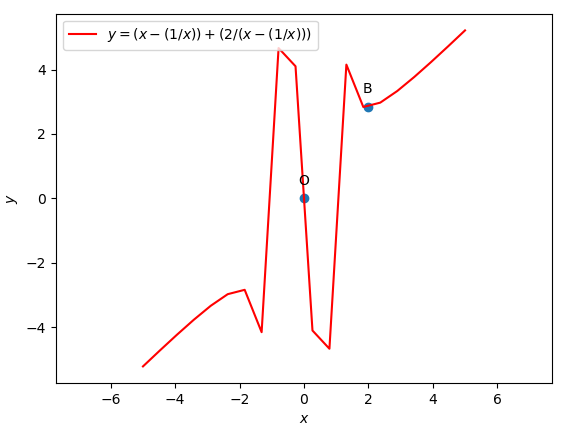
\includegraphics[width=\columnwidth]{figs/fig7.png}
	\caption{$\vec{h(x)}$ = $\frac{(x-\frac{1}{x})^2 + 2}{x-\frac{1}{x}}$}
	\label{fig:my_label}
\end{figure}
\begin{table}[h]
    \centering
    \begin{tabular}{|c|c|}
       \hline
       \textbf{Symbol}&\textbf{Value}  \\
       \hline
	    $\vec{f(x)}$ & $x^2+\frac{1}{x^2}$ \\
        \hline
	    $\vec{g(x)}$ & $x-\frac{1}{x}$\\
        \hline
	    $\vec{h(x)}$ & $\frac{\vec{f(x)}}{\vec{g(x)}}$ \\
        \hline
        x & $\in$ R-(-1,0,1)\\
        \hline
    \end{tabular}
    \caption{Given Parameters}
    \label{tab:my_label}
\end{table}
\vspace{0.3cm}
\section{Solution}
Using \textbf{Gradient descend Algorithm}, we get local minimum is 2.83

\section{Proof}
According to given conditions $\vec{h(x)}$ is expressed as,\\
\\
\begin{equation}
	\vec{h(x)} = \frac{x^2+\frac{1}{x^2}}{x-\frac{1}{x}} \label{eq-2}\\
\end{equation}
Eq-1 can be expressed as
\begin{equation}
	\vec{h(x)} = \frac{(x-\frac{1}{x})^2 + 2}{x-\frac{1}{x}} \label{eq-2}\\
\end{equation}
i.e,
\begin{equation}
	\vec{h(x)} = x-\frac{1}{x} + \frac{2}{x-\frac{1}{x}} \label{eq-3}\\
\end{equation}
\\
Differentiating on both sides,
\begin{equation}
	\vec{h'(x)} = 1+\frac{1}{x^2} - \frac{2}{(x-\frac{1}{x})^2}(1+\frac{1}{x^2})\label{eq-4}
\end{equation}
 Yielding,   \\
 \begin{equation}
	 \vec{h'(x)} = \frac{1+x^2}{(x-\frac{1}{x})^2x^4}(x^4+1-4x^2)
 \end{equation}
 \\
$\vec{h(x)}$ has a local minimum at $\vec{h'(x)} = 0$\\
\\
Therefore,
\begin{equation}
(1+x^2)(x^4+1-4x^2) = 0
\end{equation}
\\
Since,  x$\in$ R-(-1,0,1)\\
\\
Yielding,
\\
x = $\pm$1.932\\
Thus, $$\vec{h}(1.932) = 2.83$$
Therefore,\\
The minimum value of $\boldsymbol{h(x)}$ is $\boldsymbol{2.83}$
\end{document}
